


% \setlength{\tabcolsep}{9pt}
% \renewcommand{\arraystretch}{1.3}
% \begin{table*}[!htbp]
% \centering
\resizebox{\textwidth}{!}{\begin{tabular}{llcccccccc}
\toprule
 &  & \multicolumn{3}{c}{\textbf{Single-sample}} & \multicolumn{3}{c}{\textbf{Multi-sample}} & \multicolumn{2}{c}{\textbf{Other}}  \\
\cmidrule(lr){3-5} \cmidrule(lr){6-8} \cmidrule(lr){9-10}
\textbf{Category} & \textbf{Task} & \textbf{MAX} & \textbf{AVG} & \textbf{G-NLL} &  \textbf{SE}$_{EXM}$ & \textbf{DSE}$_{EXM}$ & \textbf{PE} & \textbf{P}$_{true}$ & \textbf{LEN} \\
\hline
\multirow{4}{*}{\textbf{Individual}}
& \textbf{Simple} & $0.74$ \tiny{±$.045$} & \underline{$0.76$} \tiny{±$.046$} & \best{$0.77$} \tiny{±$.045$} & $0.73$ \tiny{±$.049$} & $0.73$ \tiny{±$.049$} & $0.72$ \tiny{±$.045$} & $0.69$ \tiny{±$.052$} & $0.56$ \tiny{±$.052$} \\
& \textbf{Multiple} & $0.71$ \tiny{±$.065$} & \underline{$0.74$} \tiny{±$.066$} & \best{$0.76$} \tiny{±$.065$} & $0.73$ \tiny{±$.073$} & $0.73$ \tiny{±$.073$} & $0.71$ \tiny{±$.071$} & $0.67$ \tiny{±$.075$} & $0.58$ \tiny{±$.081$} \\
& \textbf{Parallel} & $0.66$ \tiny{±$.059$} & \best{$0.72$} \tiny{±$.058$} & \underline{$0.71$} \tiny{±$.058$} & $0.66$ \tiny{±$.059$} & $0.66$ \tiny{±$.059$} & $0.67$ \tiny{±$.061$} & $0.62$ \tiny{±$.063$} & $0.49$ \tiny{±$.064$} \\
& \textbf{Parallel-Multiple} & $0.72$ \tiny{±$.048$} & \underline{$0.74$} \tiny{±$.048$} & \best{$0.76$} \tiny{±$.048$} & $0.73$ \tiny{±$.051$} & $0.73$ \tiny{±$.051$} & $0.72$ \tiny{±$.052$} & $0.67$ \tiny{±$.059$} & $0.55$ \tiny{±$.060$} \\
\hline
\multirow{4}{*}{\textbf{Combinations}}
& \textbf{Simple + Multiple} & $0.73$ \tiny{±$.036$} & \underline{$0.75$} \tiny{±$.037$} & \best{$0.77$} \tiny{±$.037$} & $0.73$ \tiny{±$.041$} & $0.73$ \tiny{±$.041$} & $0.72$ \tiny{±$.038$} & $0.68$ \tiny{±$.042$} & $0.57$ \tiny{±$.044$} \\
& \textbf{Simple + Parallel} & $0.70$ \tiny{±$.037$} & \underline{$0.71$} \tiny{±$.039$} & \best{$0.75$} \tiny{±$.036$} & \underline{$0.71$} \tiny{±$.038$} & $0.70$ \tiny{±$.038$} & $0.67$ \tiny{±$.040$} & $0.68$ \tiny{±$.038$} & $0.59$ \tiny{±$.039$} \\
& \textbf{Multiple + Parallel-Multiple} & $0.73$ \tiny{±$.037$} & $0.71$ \tiny{±$.039$} & \best{$0.77$} \tiny{±$.037$} & \underline{$0.74$} \tiny{±$.041$} & $0.73$ \tiny{±$.041$} & $0.68$ \tiny{±$.041$} & $0.69$ \tiny{±$.045$} & $0.64$ \tiny{±$.045$} \\
        & \textbf{All Combined}  & \underline{$0.72$} \tiny{±$.026$} & $0.71$ \tiny{±$.027$} & \best{$0.76$} \tiny{±$.025$} & \underline{$0.72$} \tiny{±$.027$} & \underline{$0.72$} \tiny{±$.027$} & $0.68$ \tiny{±$.028$} & $0.68$ \tiny{±$.029$} & $0.61$ \tiny{±$.030$} \\
\hline
\multirow{2}{*}{\textbf{Unanswerable}}
& \textbf{Simple + Irrelevance} & $0.78$ \tiny{±$.026$} & \underline{$0.80$} \tiny{±$.025$} & \best{$0.81$} \tiny{±$.025$} & $0.76$ \tiny{±$.026$} & $0.76$ \tiny{±$.026$} & $0.79$ \tiny{±$.026$} & $0.76$ \tiny{±$.026$} & $0.50$ \tiny{±$.032$} \\
& \textbf{All Combined + Irrelevance} & $0.74$ \tiny{±$.020$} & \underline{$0.77$} \tiny{±$.020$} & \best{$0.78$} \tiny{±$.020$} & $0.74$ \tiny{±$.020$} & $0.74$ \tiny{±$.020$} & $0.75$ \tiny{±$.021$} & $0.71$ \tiny{±$.022$} & $0.49$ \tiny{±$.024$} \\
\bottomrule
\end{tabular}}

\caption{
\color{black} 
Results:
Mean AUROC $\pm$ mean standard error (mean over eight LLMs) for individual tasks, task combinations, and unanswerable requests described in \Cref{sec:individual_tasks}, \Cref{sec:combinations}, and \Cref{sec:irrelevance_combinations} respectively.
The best result in \best{green}, \underline{underlined} second best.
For per-LLM results, see \Cref{fig:individual_tasks,fig:combinations,fig:irrelevance_combinations}
(\Cref{app:detailed_results}).
}

% \label{tab:combined_all_tasks}
% \end{table*}







\section{Benchmarking UQ Performance in Function-Calling}
\label{sec:benchmark}

We build upon the Berkeley Function Calling Leaderboard (BFCL) benchmark \citep{bfcl}, which provides a collection of FC examples, mostly in Python with small parts in Java and JavaScript.
The BFCL benchmark consists of multiple tasks, with a separate dataset for evaluating each one of them. Beyond being able to compare different UQ methods for FC purposes, developing a UQ benchmark based on the BFCL allows for users to simultaneously evaluate model accuracy---how often the LLM is right---and model UQ---how well the model's uncertainty predicts its correctness. %

To quantify this, we evaluate how well uncertainty estimates discriminate correct from incorrect function calls in the selective prediction setting \citep{el-yaniv2010found}.
First, we determine whether a given response is correct with Abstract Syntax Tree (AST) matching w.r.t.\ the ground truth response, as default in BFCL. 
Then, the problem is interpreted as a binary classification of whether the response is correct or not, using the UQ score calculated as the classifier-score. 
The UQ-performance is then quantified as the performance of this classifier. The most appropriate metric to use for this is
the area under the receiver-operation characteristic (AUROC) \citep{fawcett2006introduction}. 
It yields a value of 0.5 for random uncertainty estimates and 1.0 for uncertainty estimates that perfectly discriminate correct from incorrect outputs. 
In \Cref{sec:risk_coverage}, we also include risk-coverage (rejection-accuracy) curves 
to illustrate what the AUROC values correspond to in terms of potential accuracy gains thanks to UQ-based abstention.



We evaluate the UQ methods of \Cref{sec:uq-methods} across eight LLMs:
Qwen2.5-\{0.5,3,7\}B-Instruct, 
Ministral-8B-Instruct-2410, Qwen3-4B-Instruct-2507, gemma-2-9b-it, and gemma-3-\{4,12\}b-it. We evaluate the correctness of the greedy decoding response (temperature $T\!=\!0$) and draw 10 samples at $T\!=\!1$ to compute the multi-sample UQ methods. We begin in \Cref{sec:individual_tasks} by directly adapting the well-defined single-turn tasks from the BFCL to measure the utility of UQ methods.
These tasks vary in difficulty, allowing to progressively test the LLMs' and UQ methods' performances on increasingly harder tasks.
Next, in \Cref{sec:combinations}, we explain why such a straightforward analysis on each individual task, while useful, is insufficient for comprehensive UQ evaluation, and present our adaptations that allow for a more realistic evaluation.
In \Cref{sec:irrelevance_combinations}, we evaluate how well the UQ methods work for requests that cannot be solved by the LLM given the available tools.


\setlength{\tabcolsep}{9pt}
\renewcommand{\arraystretch}{1.3}
\begin{table*}[!htbp]
\centering
\resizebox{\textwidth}{!}{\begin{tabular}{llcccccccc}
\toprule
 &  & \multicolumn{3}{c}{\textbf{Single-sample}} & \multicolumn{3}{c}{\textbf{Multi-sample}} & \multicolumn{2}{c}{\textbf{Other}}  \\
\cmidrule(lr){3-5} \cmidrule(lr){6-8} \cmidrule(lr){9-10}
\textbf{Category} & \textbf{Task} & \textbf{MAX} & \textbf{AVG} & \textbf{G-NLL} &  \textbf{SE}$_{EXM}$ & \textbf{DSE}$_{EXM}$ & \textbf{PE} & \textbf{P}$_{true}$ & \textbf{LEN} \\
\hline
\multirow{4}{*}{\textbf{Individual}}
& \textbf{Simple} & $0.74$ \tiny{±$.045$} & \underline{$0.76$} \tiny{±$.046$} & \best{$0.77$} \tiny{±$.045$} & $0.73$ \tiny{±$.049$} & $0.73$ \tiny{±$.049$} & $0.72$ \tiny{±$.045$} & $0.69$ \tiny{±$.052$} & $0.56$ \tiny{±$.052$} \\
& \textbf{Multiple} & $0.71$ \tiny{±$.065$} & \underline{$0.74$} \tiny{±$.066$} & \best{$0.76$} \tiny{±$.065$} & $0.73$ \tiny{±$.073$} & $0.73$ \tiny{±$.073$} & $0.71$ \tiny{±$.071$} & $0.67$ \tiny{±$.075$} & $0.58$ \tiny{±$.081$} \\
& \textbf{Parallel} & $0.66$ \tiny{±$.059$} & \best{$0.72$} \tiny{±$.058$} & \underline{$0.71$} \tiny{±$.058$} & $0.66$ \tiny{±$.059$} & $0.66$ \tiny{±$.059$} & $0.67$ \tiny{±$.061$} & $0.62$ \tiny{±$.063$} & $0.49$ \tiny{±$.064$} \\
& \textbf{Parallel-Multiple} & $0.72$ \tiny{±$.048$} & \underline{$0.74$} \tiny{±$.048$} & \best{$0.76$} \tiny{±$.048$} & $0.73$ \tiny{±$.051$} & $0.73$ \tiny{±$.051$} & $0.72$ \tiny{±$.052$} & $0.67$ \tiny{±$.059$} & $0.55$ \tiny{±$.060$} \\
\hline
\multirow{4}{*}{\textbf{Combinations}}
& \textbf{Simple + Multiple} & $0.73$ \tiny{±$.036$} & \underline{$0.75$} \tiny{±$.037$} & \best{$0.77$} \tiny{±$.037$} & $0.73$ \tiny{±$.041$} & $0.73$ \tiny{±$.041$} & $0.72$ \tiny{±$.038$} & $0.68$ \tiny{±$.042$} & $0.57$ \tiny{±$.044$} \\
& \textbf{Simple + Parallel} & $0.70$ \tiny{±$.037$} & \underline{$0.71$} \tiny{±$.039$} & \best{$0.75$} \tiny{±$.036$} & \underline{$0.71$} \tiny{±$.038$} & $0.70$ \tiny{±$.038$} & $0.67$ \tiny{±$.040$} & $0.68$ \tiny{±$.038$} & $0.59$ \tiny{±$.039$} \\
& \textbf{Multiple + Parallel-Multiple} & $0.73$ \tiny{±$.037$} & $0.71$ \tiny{±$.039$} & \best{$0.77$} \tiny{±$.037$} & \underline{$0.74$} \tiny{±$.041$} & $0.73$ \tiny{±$.041$} & $0.68$ \tiny{±$.041$} & $0.69$ \tiny{±$.045$} & $0.64$ \tiny{±$.045$} \\
        & \textbf{All Combined}  & \underline{$0.72$} \tiny{±$.026$} & $0.71$ \tiny{±$.027$} & \best{$0.76$} \tiny{±$.025$} & \underline{$0.72$} \tiny{±$.027$} & \underline{$0.72$} \tiny{±$.027$} & $0.68$ \tiny{±$.028$} & $0.68$ \tiny{±$.029$} & $0.61$ \tiny{±$.030$} \\
\hline
\multirow{2}{*}{\textbf{Unanswerable}}
& \textbf{Simple + Irrelevance} & $0.78$ \tiny{±$.026$} & \underline{$0.80$} \tiny{±$.025$} & \best{$0.81$} \tiny{±$.025$} & $0.76$ \tiny{±$.026$} & $0.76$ \tiny{±$.026$} & $0.79$ \tiny{±$.026$} & $0.76$ \tiny{±$.026$} & $0.50$ \tiny{±$.032$} \\
& \textbf{All Combined + Irrelevance} & $0.74$ \tiny{±$.020$} & \underline{$0.77$} \tiny{±$.020$} & \best{$0.78$} \tiny{±$.020$} & $0.74$ \tiny{±$.020$} & $0.74$ \tiny{±$.020$} & $0.75$ \tiny{±$.021$} & $0.71$ \tiny{±$.022$} & $0.49$ \tiny{±$.024$} \\
\bottomrule
\end{tabular}}

\caption{
\color{black} 
Results:
Mean AUROC $\pm$ mean standard error (mean over eight LLMs) for individual tasks, task combinations, and unanswerable requests described in \Cref{sec:individual_tasks}, \Cref{sec:combinations}, and \Cref{sec:irrelevance_combinations} respectively.
The best result in \best{green}, \underline{underlined} second best.
For per-LLM results, see \Cref{fig:individual_tasks,fig:combinations,fig:irrelevance_combinations}
(\Cref{app:detailed_results}).
}

\label{tab:combined_all_tasks}
\end{table*}



\subsection{How well do the UQ Methods Work for Individual Tasks?}
\label{sec:individual_tasks}
First, we evaluate how well the UQ methods work when we individually consider the tasks defined in BFCL.
To this end, we use the following individual Python task datasets from BFCL in their standard form: 
\emph{Simple}\footnote{BFCL's Simple split consists of 3 parts: Python, Java, and JavaScript. To be able to compare with the other three Python-based tasks (which do not have Java \& Javascript counterparts), we focus on the Python part of Simple.},
\emph{Multiple}, \emph{Parallel}, and \emph{Parallel-Multiple}.
\emph{Simple} consists of 400 requests where only one function is made available to the LLM. 
It tests whether the model is able to call the function provided, together with the correct argument values, to solve the request.
\emph{Multiple} provides definitions of multiple functions and tests whether the model can choose the correct function as well as their correct arguments to solve the request (200 requests). 
\emph{Parallel} requires the model to call multiple functions in parallel, including their correct arguments (200 requests). 
Like in \emph{Simple}, the model is only provided with the functions it needs to use.
\emph{Parallel-Multiple} combines the challenges of \emph{Parallel} and \emph{Multiple}: 
the model is provided with multiple functions, some of which are unnecessary to solve the request.
The model needs to choose which functions to call, and set their parameters correctly (200 requests).
Importantly, all of the requests in these four tasks are solvable given the functions provided as part of the request.

\begin{figure}[h!]
\centering
\begin{tikzpicture}[
  font=\small,
  box/.style={draw, rounded corners=2pt, minimum width=3.05cm, minimum height=1.05cm, align=center, thick},
  lbl/.style={font=\small\itshape},
]
% axis arrows
\draw[->, thick] (-0.35,-0.35) -- (-0.35,2.85) node[midway, above, rotate=90, yshift=6pt, lbl] {\# functions provided (A)};
\draw[->, thick] (-0.35,-0.35) -- (7.0,-0.35) node[midway, below, yshift=-2pt, lbl] {\# calls required (B)};
% quadrants
\node[box, fill=cyan5]   at (1.4,0.4) {\textbf{Simple}\\[-1pt]{\footnotesize 1 function, 1 call}};
\node[box, fill=blue4]   at (5.0,0.4) {\textbf{Parallel}\\[-1pt]{\footnotesize 1 function, $n$ calls}};
\node[box, fill=green3]  at (1.4,2.1) {\textbf{Multiple}\\[-1pt]{\footnotesize $m$ functions, 1 call}};
\node[box, fill=yellow2] at (5.0,2.1) {\textbf{Parallel-Multiple}\\[-1pt]{\footnotesize $m$ functions, $n$ calls}};
% irrelevance
\node[box, fill=pink1, minimum width=3.05cm] at (10.0,1.25) {\textbf{Irrelevance}\\[-1pt]{\footnotesize 1 insufficient function,}\\[-2pt]{\footnotesize correct action: refuse}};
\draw[dashed, thick] (8.05,-0.5) -- (8.05,3.0);
\node[lbl] at (10.0,-0.35) {unanswerable};
\node[lbl] at (3.2,3.15) {answerable};
\end{tikzpicture}
\caption{The BFCL task regimes we evaluate, arranged along the two axes we vary: the number of functions made available in the request (A) and the number of calls needed to satisfy it (B). \emph{Irrelevance} sits outside this grid, since the provided function is insufficient and the correct behaviour is to emit no call at all. \Cref{sec:combinations} combines the four answerable regimes to obtain multi-modal task distributions, and \Cref{sec:irrelevance_combinations} adds \emph{Irrelevance}.}
\label{fig:regimes}
\end{figure}

Throughout our analysis, we exclude the requests for which the greedy decoding results in an output that could not be interpreted by the Python interpreter, i.e., that result in an Abstract Syntax Tree (AST) decoding error.
These cases are clearly incorrect since they do not produce valid function calls, but also since they do not result in an execution, they cannot cause irreversible undesired outcomes.
In a practical context, we would thus not need model uncertainty to flag potentially erroneous function calls for these cases.
These errors are rare (on average $3.4\%$ of outputs on the \emph{All Combined} split), and including them does not change the relative ranking of UQ methods (Spearman correlation $0.94$); see \Cref{app:ast_errors} for effective sample sizes per model and further details.

In \Cref{tab:combined_all_tasks} (top), we report the mean (over eight LLMs) AUROC for each combination of task and UQ method, along with the mean of the per-LLM standard error.
Standard errors imply a confidence interval on the mean AUROC value, and were estimated via bootstrap sampling with 1000 samples.
\Cref{fig:individual_tasks} of \Cref{app:detailed_results} breaks down the results in \Cref{tab:combined_all_tasks} to show the per-model performances.

The results show that the sequence likelihood (G-NLL) %
generally performs best (often by a small margin)
and outperforms the entropy-based multi-sample methods we evaluate.
Overall, the level of performance achieved by the best methods on these individual tasks (AUROC of $\sim 0.7-0.8$) resembles the performance achieved by these methods on natural language Q\&A tasks \citep{aichberger2024rethi,farquhar2024detec}.





\subsection{How well do UQ Methods Work on more 
Realistic Multi-Modal Task Distributions? }
\label{sec:combinations}
In accuracy-oriented evaluation, it is possible to evaluate a model on individual tasks and then obtain a valid estimator of the mixture's performance by averaging the individual task performance estimates, weighted by the mixture's component weights, because accuracy is a linear metric.

However, unlike accuracy, AUROC measures ranking performance rather than raw correctness counts, and so is not a linear metric.
This implies that if we consider a mixture of multiple different task distributions, we might obtain a lower AUROC performance than for any individual task alone. This is important when using a confidence threshold to decide whether to execute a function call; in general, it would not be practical to set a different threshold for different modes of the task distribution.
For this reason, unlike in the accuracy-oriented benchmarks like BFCL, in order to estimate the UQ performance in a way that informs practical applications, we need to evaluate the UQ methods on more complex, multi-modal data distributions.
To this end, we combine the individual BFCL task data sets described in \Cref{sec:individual_tasks} into four multi-modal combinations, and evaluate the UQ methods on each of these combinations.

The four BFCL tasks we consider offer an opportunity to gradually increase the multi-modality of the input- and output- distributions along two axes:
A) number of functions at the model's disposal;
B)~number of function calls the model has to produce in order to solve the task.
\textit{Simple+Multiple} vary A, while keeping B fixed at 1.
\textit{Simple+Parallel} vary B between 1 and 2, while A is always kept at 1, i.e.\ only the function the request actually needs is provided; in \emph{Parallel} this is a single function that has to be called several times.
\textit{Multiple+Parallel-Multiple} is analogous to \textit{Simple+Parallel} in B, but with A set to a larger number such that there are always some unnecessary functions present in the input.
\textit{All Combined} combines both axes of variation, yielding the most heterogeneous of the four combinations we evaluate.%


We present the results in \Cref{tab:combined_all_tasks} (middle) and \Cref{fig:combinations}.
At a high level, the results are similar to the individual task results: G-NLL performs best out of all of the considered methods, and on average, performance levels remain roughly the same as those observed in \Cref{sec:individual_tasks}.








\subsection{Do UQ Methods Allow for Identifying Requests that are Impossible to Answer?}
\label{sec:irrelevance_combinations}

Beyond the four task datasets introduced in \Cref{sec:individual_tasks}, the BFCL benchmark also includes an \emph{Irrelevance} task to test whether models can recognize and explicitly communicate when they are not able to solve the task given the provided functions. 
Each request in this task includes a single function definition, which is not sufficient to solve the request. 
Thus, a successful answer by the model for this task consists of refusing to output any function call. 
Note that a model is able to get perfect accuracy on this task by always refusing (independent of the request). 
Hence, evaluating on this task alone can yield misleading results about UQ methods. 
We thus combine \emph{Irrelevance} with the other tasks, once with the \emph{Simple} data only (\emph{Simple + Irrelevance}), and once with all other datasets combined (\emph{All Combined + Irrelevance}). %

We present the results in \Cref{tab:combined_all_tasks} (bottom) and \Cref{fig:irrelevance_combinations}.
Again, we observe good and broadly comparable performance of most UQ methods. 
We also find that the single-sample methods (G-NLL, AVG) slightly outperform the multi-sample methods (SE$_{EXM}$, DSE$_{EXM}$, PE).







\subsection{Are UQ Methods Calibrated for FC?}
\label{sec:calibration}


% \begin{wrapfigure}[17]{r}{0.45\linewidth}
%     \centering
%     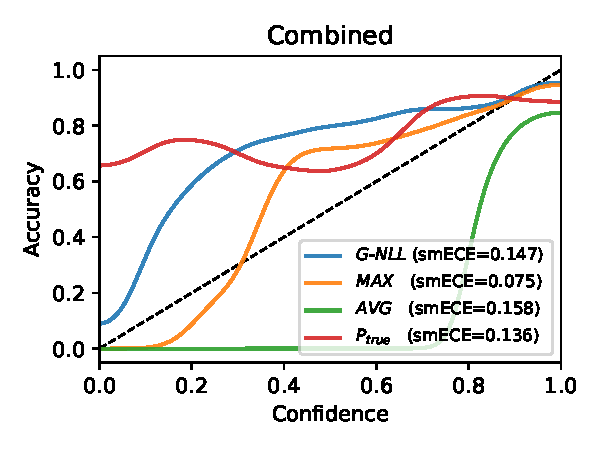
\includegraphics[width=\linewidth, trim=10 13 10 25, clip]{figures/ece/calibaration_figure_v2.pdf}
%     \caption{SmoothECE for \textit{All Combined} task, aggregated over all models.}
%     \label{fig:calibration}
% \end{wrapfigure}

Beyond being able to distinguish incorrect from correct outputs, which we have measured with AUROC in the previous sections, a desirable quality of a UQ score is to be calibrated, 
i.e., to correctly predict the probability of a sample being correct, which is important in decision-making settings \citep{kiyani2025robustdecisionmakingpartially}. 
Among several calibration measures proposed, we choose smoothECE \citep{blasiok2023smooth}, which is a smoothed version of expected calibration error (ECE) that does not exhibit discontinuous behavior. 

\begin{wrapfigure}[17]{r}{0.45\linewidth}
    \centering
    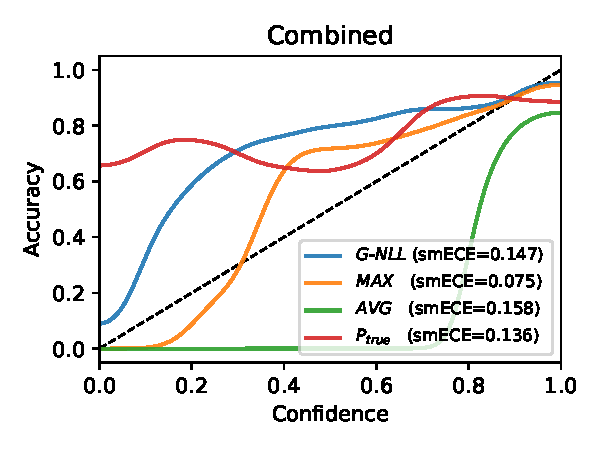
\includegraphics[width=\linewidth, trim=10 13 10 25, clip]{figures/ece/calibaration_figure_v2.pdf}
    \caption{SmoothECE for \textit{All Combined} task, aggregated over all models.}
    \label{fig:calibration}
\end{wrapfigure}

Since not all of the UQ methods we evaluate yield a valid probability score, we can only evaluate calibration for the following subset:  {MAX}, {AVG}, {G-NLL}, and {P}$_{true}$. 
In \Cref{fig:calibration}, we show the results for the \textit{All Combined} task as representative for all tasks. 
While quantitative results differ per task, qualitatively, they stay largely the same across tasks, so we relegate the detailed plots to \Cref{app:calibration}.

We make several observations. 
Firstly, {AVG} achieves the worst calibration among all methods, being largely overconfident with confidence values (x-axis) being higher than the accuracy (y-axis).
{P}$_{true}$ and {G-NLL}, on the other hand, are underconfident, as indicated by their confidence being mostly lower than the accuracy. 
For {G-NLL}, this would be expected from natural language, where the multiplication of per-token probabilities, each $<1$, tends to lead to small sequence probabilities. 
However, in function calling, this phenomenon is not as extreme since most probabilities are $\approx 1.0$ (\Cref{sec:discussion_se}). 
Lastly, {MAX} achieves the best calibration. 
It is still slightly underconfident for most parts, but since by definition $\max_i \log p_i \geq \sum_i \log p_i$, it is less underconfident than {G-NLL}, especially in low-confidence regions.
These insights complement the previous AUROC results, and illustrate that ECE does not necessarily correlate with AUROC.\footnote{For another illustrative example, consider the extreme case of a model with accuracy $0.5$ for which a UQ method assigns a correctness probability of $0.5$ for all samples. It has a perfect ECE of $0$ but an AUROC of $0.5$.}
In the setting of selective prediction---generating a function call with an option to abstain---the crucial property to assess is the ability to discriminate between correct and incorrect outputs, which is measured by AUROC. ECE measures whether confidence values are calibrated as probabilities, which is a secondary consideration in this context. Furthermore, all multi-sample entropy-based methods do not output probabilities, and hence their calibration cannot be evaluated.
We note that for methods with high AUROC but poor calibration, post-hoc calibration techniques (e.g., Platt scaling) can be applied to improve calibration without affecting discriminative performance.
We make this precise in \Cref{app:posthoc}: all of the discrimination and selective-prediction metrics we report depend on the scores only through the ranking they induce, so a strictly monotone recalibration of the score leaves them invariant. Post-hoc calibration therefore changes \emph{how} a score should be thresholded, but not \emph{which} score is preferable. \Cref{app:posthoc} also discusses which of the evaluated methods are amenable to it.


\subsection{From AUROC to Abstention}
\label{sec:selective_prediction}

AUROC measures how well a UQ score ranks correct above incorrect function calls, but it does not by itself say how much accuracy a system gains by declining to execute the calls it is least sure about. Since this is the quantity a practitioner cares about, we summarize it here and relegate the full results to \Cref{sec:risk_coverage} and \Cref{app:selection_pred_metrics}.

\Cref{fig:riskcoverage_main} shows risk-coverage curves for \emph{All Combined} and for \emph{All Combined + Irrelevance}, averaged over models. Abstaining on the $30\%$ of requests with the highest uncertainty raises accuracy from ${<}92\%$ to $96\%$ on \emph{Simple} and from $79\%$ to $86\%$ on \emph{Parallel-Multiple}, and by roughly $10$ percentage points on the splits that include \emph{Irrelevance} (\Cref{sec:risk_coverage}). UQ-based abstention is therefore not a marginal effect in this setting.

\Cref{tab:selective_main} compares the four headline methods on \emph{All Combined} under AUROC and under two selective-prediction metrics: the normalized area under the risk-coverage curve (NAURC, lower is better) and the prediction-rejection ratio at a $30\%$ and $50\%$ rejection rate (PRR, higher is better); both are defined in \Cref{app:selection_pred_metrics}. Three points stand out. First, the ordering of the single- and multi-sample families is the same under all four metrics, so our main conclusion does not depend on the choice of metric. Second, the two FC-adapted variants are the best in their respective families throughout. Third, the metrics are not redundant: at a $30\%$ rejection rate SE$_{AST}$ overtakes plain G-NLL, which the AUROC column does not reveal, and it is the FC-adapted single-sample score G-NLL$_{SMT}$ that closes that gap. We return to this in \Cref{app:selection_pred_metrics}.

\begin{table}[h!]
\centering
\scalebox{\tablescale}{
\begin{tabular}{lcccc}
\toprule
\textbf{Method} & \textbf{AUROC} $\uparrow$ & \textbf{NAURC} $\downarrow$ & \textbf{PRR@30\%} $\uparrow$ & \textbf{PRR@50\%} $\uparrow$ \\
\midrule
G-NLL & $0.76$ & $0.37$ & $0.40$ & $0.46$ \\
\textbf{G-NLL}$_{SMT}$ & \best{$0.78$} & \best{$0.35$} & \best{$0.44$} & \best{$0.51$} \\
\midrule
SE$_{EXM}$ & $0.72$ & $0.53$ & $0.38$ & $0.41$ \\
\textbf{SE}$_{AST}$ & $0.74$ & $0.52$ & $0.43$ & $0.45$ \\
\bottomrule
\end{tabular}
}
\caption{The two best single-sample and two best multi-sample methods on \emph{All Combined}, under AUROC and the selective-prediction metrics of \Cref{app:selection_pred_metrics} (mean over eight LLMs). Arrows indicate the direction of improvement; best result in \best{green}. Per-split results for all methods are in \Cref{tab:combined_all_tasks} and \Cref{tab:naurc,tab:prr30,tab:prr50}.}
\label{tab:selective_main}
\end{table}

\begin{figure*}[h!]
    \centering
    \begin{subfigure}[c]{0.48\textwidth}
        \centering
        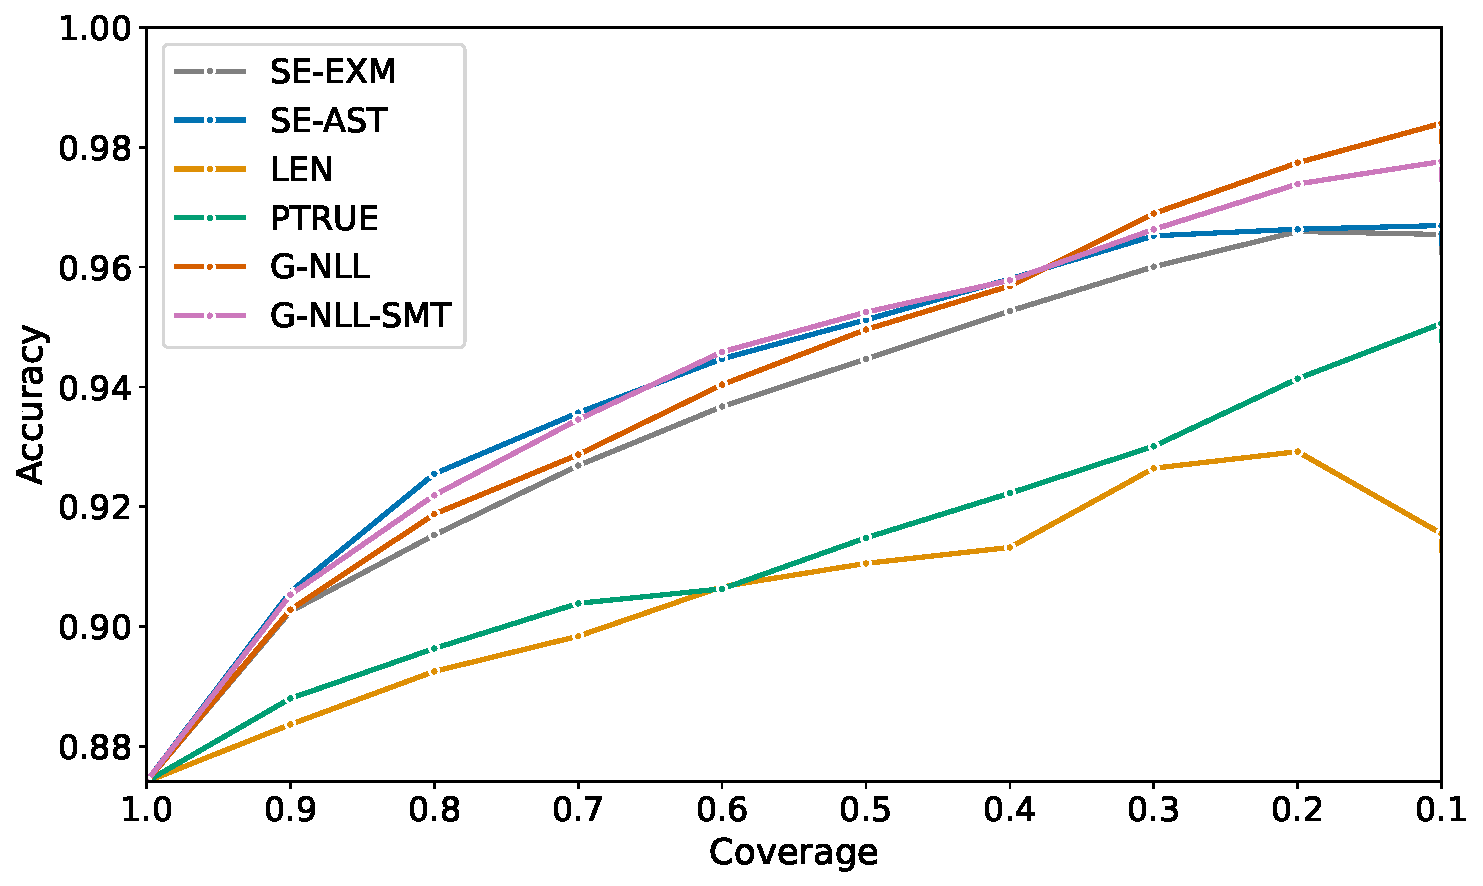
\includegraphics[width=\textwidth]{figures/rejection/simple-multiple-parallel-parallel_multiple_selective_accuracy_mean.pdf}
        \caption{All Combined}
        \label{fig:rc_main_all}
    \end{subfigure}
    \hfill
    \begin{subfigure}[c]{0.48\textwidth}
        \centering
        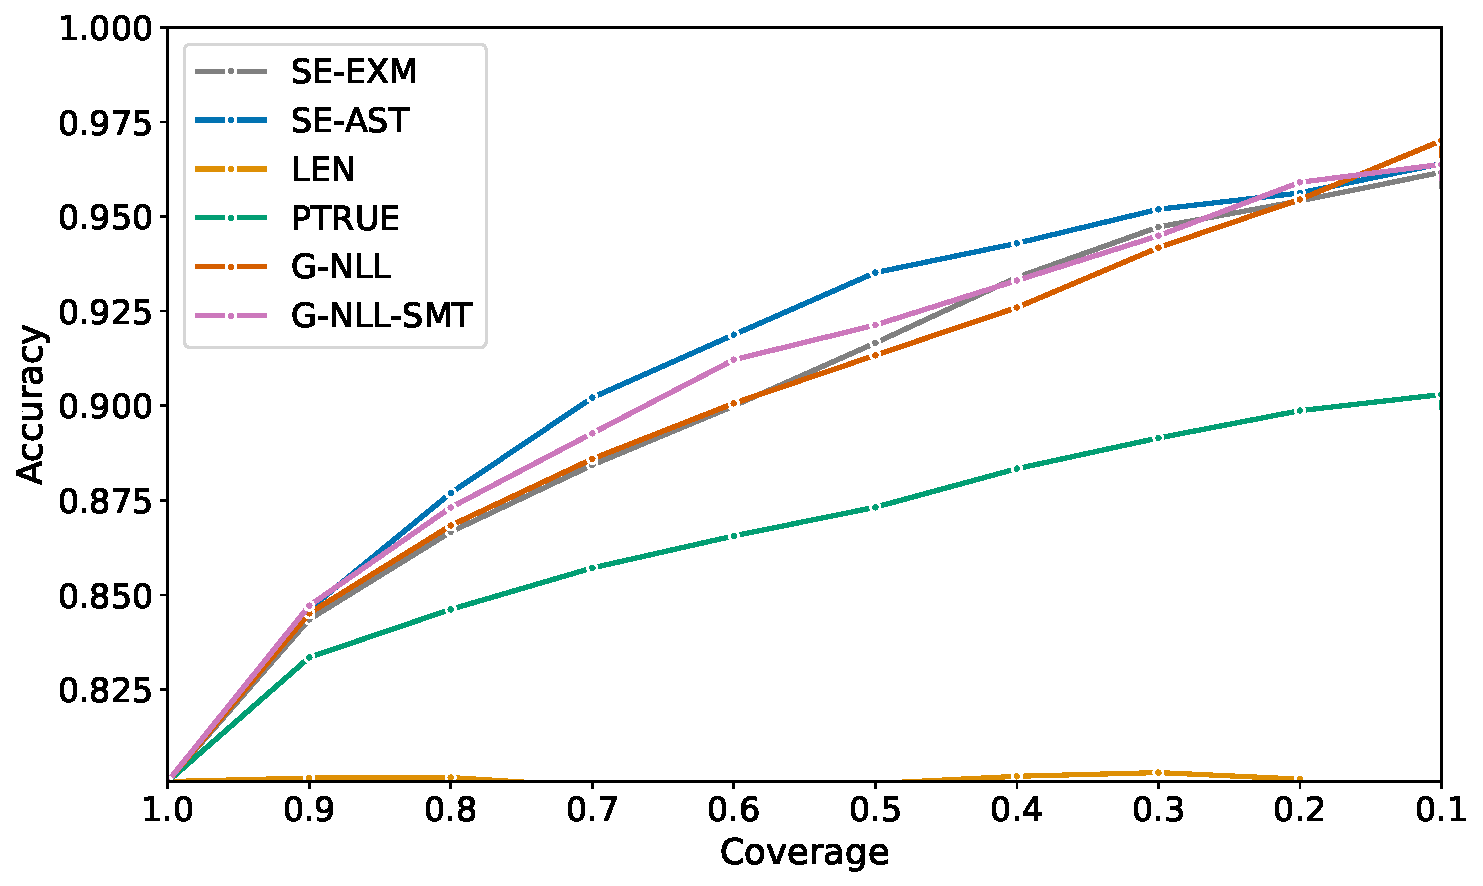
\includegraphics[width=\textwidth]{figures/rejection/simple-multiple-parallel-parallel_multiple-irrelevance_selective_accuracy_mean.pdf}
        \caption{All Combined + Irrelevance}
        \label{fig:rc_main_allirr}
    \end{subfigure}
    \caption{Risk-coverage curves on the two largest splits, averaged over the eight LLMs. Higher is better. The full set of splits is in \Cref{sec:risk_coverage}.}
    \label{fig:riskcoverage_main}
\end{figure*}
